\documentclass{article}
\usepackage{geometry}
\usepackage[section]{placeins}
\usepackage{varioref}
\usepackage{titlesec}

\geometry{letterpaper,margin=1in}

\usepackage{tikz}
\usetikzlibrary{
    positioning,
    backgrounds,
	shapes.geometric,
    patterns.meta,
    arrows.meta,
	decorations.pathreplacing,
    bending
    }

\begin{document}

\title{Eden's Promise: Eternity (Savage)\\\emph{Junction Shiva}}
\author{}
\maketitle

\section{Initial positioning}
\newcommand{\sectionbreak}{\clearpage}
The party splits up into the usual tank-healer-DPS-DPS groups.  Healer 1's group (G1) will tend slightly southeast of the boss, and Healer 2's group (G2) will be opposite them to the northwest (figure \vref{initpos}).  In the next step of the mechanic, the inner circle and six of the outer circles will be marked with AOEs.  Each group will go to the safe spot on their side of the dotted line.

\begin{figure}[h]
	\centering
	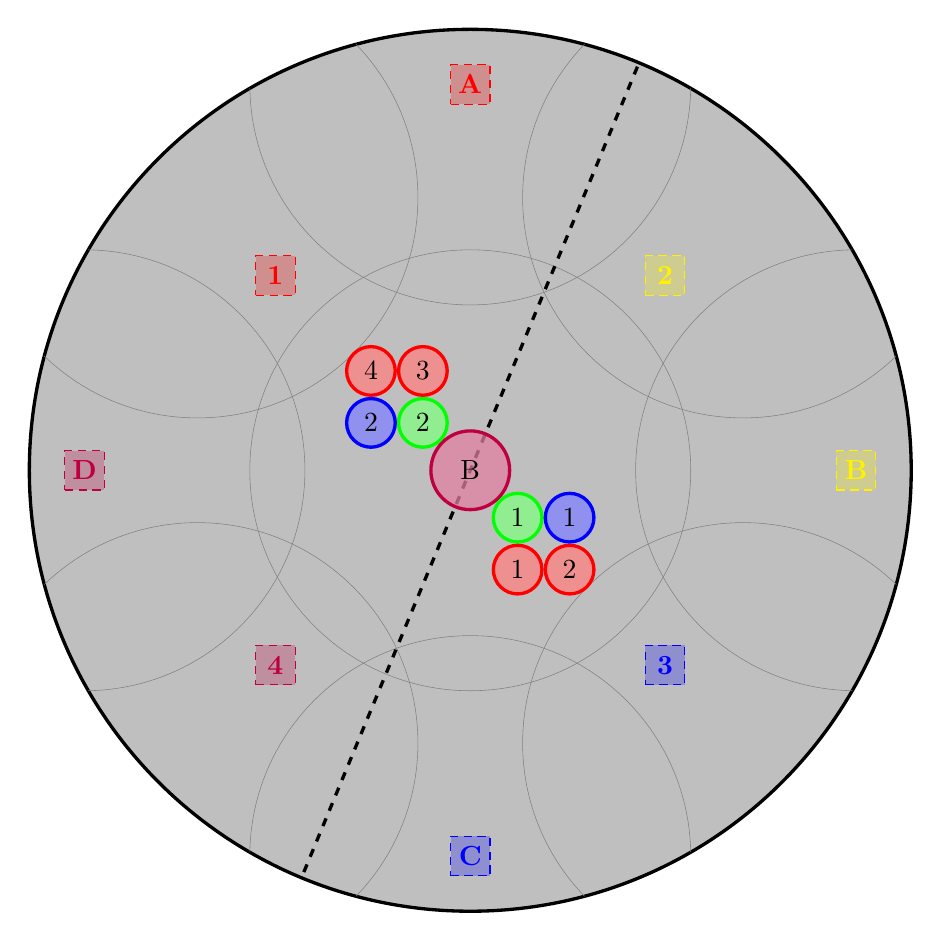
\begin{tikzpicture}[scale=1.4, every pic/.style=[transform shape]]
		% chktex-file 1
% chktex-file 8
\tikzset{arena/.style =
        {
            very thick,
            fill=gray,
            fill opacity=0.5
        }
}

\tikzset {marker/.style =
        {
            rectangle,
            densely dashed,
            minimum size=0.5cm,
            inner sep=0cm,
            text opacity=1,
            draw
        }
}

\tikzset{aoe/.style =
        {
            thick,
            orange,
            pattern={
                    Lines[angle=45, distance=0.5cm, line width=0.25cm]
                },
            pattern color=yellow,
            opacity=0.25,
            draw opacity=1
        }
}

\tikzset{aoe fill/.style = {
            fill=red,
            opacity=0.25
        }
}

\tikzset{cone aoe/.pic = {
            \draw [preaction={aoe fill}] [aoe] (0,0) -- (#1/2:10) arc (#1:-1*#1:5) -- cycle;
        }
}

\tikzset{line aoe/.pic = {
            \draw [preaction={aoe fill}] [aoe] (0,-0.5*#1) rectangle (10,0.5*#1);
        }
}

\tikzset{circle aoe/.pic = {
            \draw [preaction={aoe fill}] [aoe] (0,0) circle [radius=#1];
        }
}

\tikzset{pics/donut aoe/.style 2 args = {
            code = {
                    \draw [preaction={even odd rule,aoe fill}] [even odd rule,aoe] (0,0) circle [radius=#1] circle [radius=#2];
                }
        }
}

\tikzset{boss/.style =
        {
            shape=circle,
            very thick,
            purple,
            fill=purple!50,
            fill opacity=0.75,
            minimum size=1cm,
            text=black,
            text opacity=1,
            draw
        }
}

\tikzset{tank/.style =
        {
            boss,
            draw=blue,
            fill=blue!50,
            minimum size=0.5cm
        }
}

\tikzset{dps/.style =
        {
            tank,
            draw=red,
            fill=red!50
        }
}

\tikzset{heal/.style =
        {
            tank,
            draw=green,
            fill=green!50
        }
}

\tikzset{endat/.style =
        {
            shape=circle,
            very thick,
            draw=black,
            fill=black!50,
            minimum size=0.5cm
        }
}

\tikzset{startat/.style =
        {
            endat,
            dashed
        }
}

\tikzset{nf/.style = { fill=none } }

\tikzset{move/.style = {
            line width=2pt,
            -Latex,
            fill=none
        }
}

\tikzset{tether/.style = {
        line width=2pt,
        purple,
        dotted,
        -Latex,
        text=black
    }
}

\tikzset{icicle/.style =
        {
            shape=diamond,
            very thick,
            cyan,
            fill=cyan!50,
            fill opacity=0.75,
            minimum size=1cm,
            text=black,
            text opacity=1,
            draw
        }
}
		\node[boss] (boss) at (0,0) {B};

		\node[heal, below right=0cm of boss] (h1) {1};
		\node[heal, above left=0cm of boss] (h2) {2};
		\node[tank, right=0cm of h1] (t1) {1};
		\node[tank, left=0cm of h2] (t2) {2};
		\node[dps, below=0cm of h1] (d1) {1};
		\node[dps, below=0cm of t1] (d2) {2};
		\node[dps, above=0cm of h2] (d3) {3};
		\node[dps, above=0cm of t2] (d4) {4};

		\foreach \letter / \ang / \rad / \c in
			{A/90/3.5/red,
				D/180/3.5/purple,
				C/270/3.5/blue,
				B/0/3.5/yellow,
				1/135/2.5/red,
				4/225/2.5/purple,
				3/315/2.5/blue,
				2/45/2.5/yellow}
		\node[marker, color=\c, fill, fill opacity=0.25] at (\ang:\rad) (marker-\letter) {\textbf\letter};

		\begin{scope}[on background layer]
			\draw[arena] (0,0) circle [radius=4];
			\clip (0,0) circle [radius=4];
			\draw[help lines] (0,0) circle [radius=2];
			\foreach \ang in {0, 45,...,315}
			\draw[help lines] (\ang:3.5) circle [radius=2];
			\draw[very thick, dashed] (247.5:5) -- (67.5:5);
		\end{scope}

	\end{tikzpicture}
	\caption{The initial position; the dotted line across the arena indicates each group's possible position assignments for the next step}
	\label{initpos}
\end{figure}

\section{First slide}

The platform freezes.  Each party member identifies the safe spot on their side of the arena and slides into it (figure \vref{firstslide}), waiting for the stack marker on the healer to resolve.

In this example, the safe spots are at 2 and 4, but they can be at any pair of locations opposite each other.

\begin{figure}[h]
	\centering
	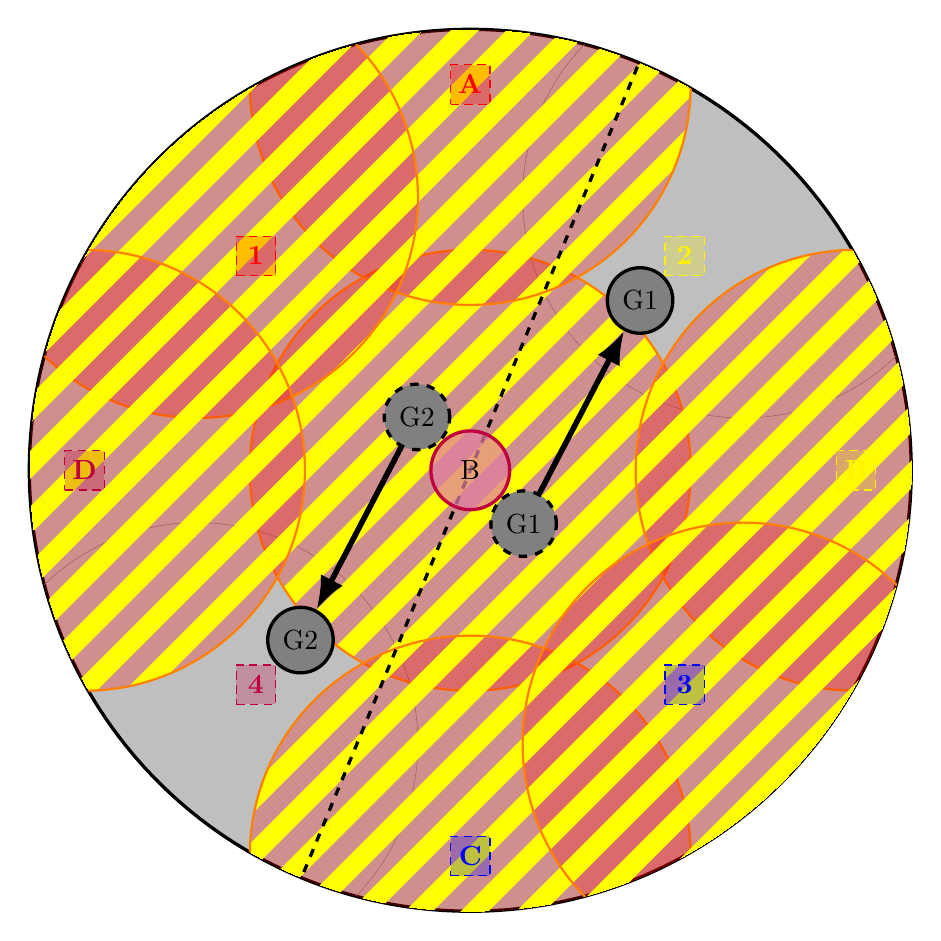
\begin{tikzpicture}[scale=1.4, every pic/.style={scale=1.4, transform shape}]
		% chktex-file 1
% chktex-file 8
\tikzset{arena/.style =
        {
            very thick,
            fill=gray,
            fill opacity=0.5
        }
}

\tikzset {marker/.style =
        {
            rectangle,
            densely dashed,
            minimum size=0.5cm,
            inner sep=0cm,
            text opacity=1,
            draw
        }
}

\tikzset{aoe/.style =
        {
            thick,
            orange,
            pattern={
                    Lines[angle=45, distance=0.5cm, line width=0.25cm]
                },
            pattern color=yellow,
            opacity=0.25,
            draw opacity=1
        }
}

\tikzset{aoe fill/.style = {
            fill=red,
            opacity=0.25
        }
}

\tikzset{cone aoe/.pic = {
            \draw [preaction={aoe fill}] [aoe] (0,0) -- (#1/2:10) arc (#1:-1*#1:5) -- cycle;
        }
}

\tikzset{line aoe/.pic = {
            \draw [preaction={aoe fill}] [aoe] (0,-0.5*#1) rectangle (10,0.5*#1);
        }
}

\tikzset{circle aoe/.pic = {
            \draw [preaction={aoe fill}] [aoe] (0,0) circle [radius=#1];
        }
}

\tikzset{pics/donut aoe/.style 2 args = {
            code = {
                    \draw [preaction={even odd rule,aoe fill}] [even odd rule,aoe] (0,0) circle [radius=#1] circle [radius=#2];
                }
        }
}

\tikzset{boss/.style =
        {
            shape=circle,
            very thick,
            purple,
            fill=purple!50,
            fill opacity=0.75,
            minimum size=1cm,
            text=black,
            text opacity=1,
            draw
        }
}

\tikzset{tank/.style =
        {
            boss,
            draw=blue,
            fill=blue!50,
            minimum size=0.5cm
        }
}

\tikzset{dps/.style =
        {
            tank,
            draw=red,
            fill=red!50
        }
}

\tikzset{heal/.style =
        {
            tank,
            draw=green,
            fill=green!50
        }
}

\tikzset{endat/.style =
        {
            shape=circle,
            very thick,
            draw=black,
            fill=black!50,
            minimum size=0.5cm
        }
}

\tikzset{startat/.style =
        {
            endat,
            dashed
        }
}

\tikzset{nf/.style = { fill=none } }

\tikzset{move/.style = {
            line width=2pt,
            -Latex,
            fill=none
        }
}

\tikzset{tether/.style = {
        line width=2pt,
        purple,
        dotted,
        -Latex,
        text=black
    }
}

\tikzset{icicle/.style =
        {
            shape=diamond,
            very thick,
            cyan,
            fill=cyan!50,
            fill opacity=0.75,
            minimum size=1cm,
            text=black,
            text opacity=1,
            draw
        }
}
		\foreach \letter / \ang / \rad / \c in
			{A/90/3.5/red,
				D/180/3.5/purple,
				C/270/3.5/blue,
				B/0/3.5/yellow,
				1/135/2.75/red,
				4/225/2.75/purple,
				3/315/2.75/blue,
				2/45/2.75/yellow}
		\node[marker, color=\c, fill, fill opacity=0.25] at (\ang:\rad) (marker-\letter) {\textbf\letter};

		\node[boss] (boss) at (0,0) {B};

		\begin{scope}[name prefix=X]
			\node[startat, below right=0cm of boss] (g1) {G1};
			\node[startat, above left=0cm of boss] (g2) {G2};
		\end{scope}

		\node[endat, below left=0cm of marker-2] (g1) {G1};
		\node[endat, above right=0cm of marker-4] (g2) {G2};

		\begin{scope}[on background layer, transparency group]
			\draw[arena] (0,0) circle [radius=4];
			\clip (0,0) circle [radius=4];

			\foreach \ang in {0, 45,...,315}
			\draw[help lines] (\ang:3.5) circle [radius=2];
			\begin{scope}[transparency group]
				\pic at (0,0) {circle aoe=2cm};
				\foreach \ang in {0, 90, 135, 180, 270, 315}
				\pic at (\ang:3.5) {circle aoe=2cm};
			\end{scope}
			\draw[very thick, dashed] (247.5:5) -- (67.5:5);
		\end{scope}

		\draw[move] (Xg1) -- (g1);
		\draw[move] (Xg2) -- (g2);

	\end{tikzpicture}
	\caption{Sliding to the safe spot and stacking to resolve the marker}
	\label{firstslide}
\end{figure}

\section{Second slide}

The platform remains frozen.  All the current AOEs resolve and the final two circles are now targeted for AOEs.  Each group fans out from their current position (figure \vref{secondslide}).  Each player will be targeted with an icicle that deals PBAOE damage at the beginning of the next step, so it is required that no two players end up close enough to overlap.

\begin{figure}[h]
	\centering
	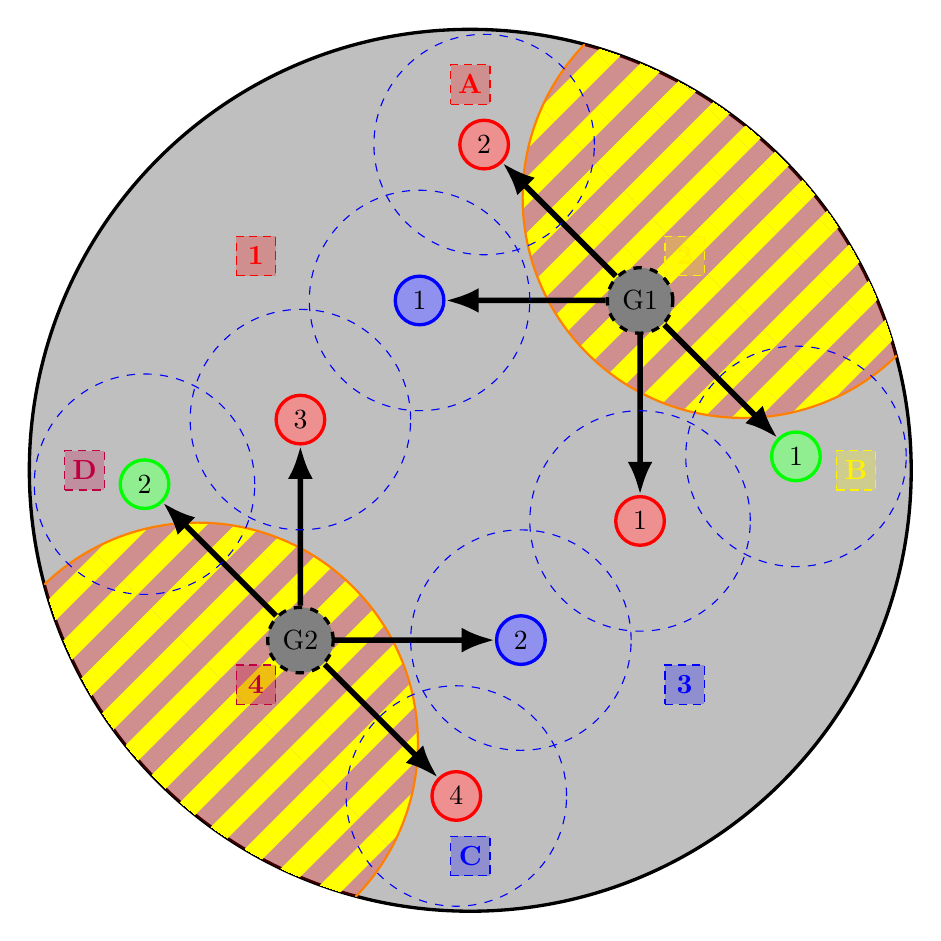
\begin{tikzpicture}[scale=1.4, every pic/.style={scale=1.4, transform shape}]
		% chktex-file 1
% chktex-file 8
\tikzset{arena/.style =
        {
            very thick,
            fill=gray,
            fill opacity=0.5
        }
}

\tikzset {marker/.style =
        {
            rectangle,
            densely dashed,
            minimum size=0.5cm,
            inner sep=0cm,
            text opacity=1,
            draw
        }
}

\tikzset{aoe/.style =
        {
            thick,
            orange,
            pattern={
                    Lines[angle=45, distance=0.5cm, line width=0.25cm]
                },
            pattern color=yellow,
            opacity=0.25,
            draw opacity=1
        }
}

\tikzset{aoe fill/.style = {
            fill=red,
            opacity=0.25
        }
}

\tikzset{cone aoe/.pic = {
            \draw [preaction={aoe fill}] [aoe] (0,0) -- (#1/2:10) arc (#1:-1*#1:5) -- cycle;
        }
}

\tikzset{line aoe/.pic = {
            \draw [preaction={aoe fill}] [aoe] (0,-0.5*#1) rectangle (10,0.5*#1);
        }
}

\tikzset{circle aoe/.pic = {
            \draw [preaction={aoe fill}] [aoe] (0,0) circle [radius=#1];
        }
}

\tikzset{pics/donut aoe/.style 2 args = {
            code = {
                    \draw [preaction={even odd rule,aoe fill}] [even odd rule,aoe] (0,0) circle [radius=#1] circle [radius=#2];
                }
        }
}

\tikzset{boss/.style =
        {
            shape=circle,
            very thick,
            purple,
            fill=purple!50,
            fill opacity=0.75,
            minimum size=1cm,
            text=black,
            text opacity=1,
            draw
        }
}

\tikzset{tank/.style =
        {
            boss,
            draw=blue,
            fill=blue!50,
            minimum size=0.5cm
        }
}

\tikzset{dps/.style =
        {
            tank,
            draw=red,
            fill=red!50
        }
}

\tikzset{heal/.style =
        {
            tank,
            draw=green,
            fill=green!50
        }
}

\tikzset{endat/.style =
        {
            shape=circle,
            very thick,
            draw=black,
            fill=black!50,
            minimum size=0.5cm
        }
}

\tikzset{startat/.style =
        {
            endat,
            dashed
        }
}

\tikzset{nf/.style = { fill=none } }

\tikzset{move/.style = {
            line width=2pt,
            -Latex,
            fill=none
        }
}

\tikzset{tether/.style = {
        line width=2pt,
        purple,
        dotted,
        -Latex,
        text=black
    }
}

\tikzset{icicle/.style =
        {
            shape=diamond,
            very thick,
            cyan,
            fill=cyan!50,
            fill opacity=0.75,
            minimum size=1cm,
            text=black,
            text opacity=1,
            draw
        }
}
		\foreach \letter / \ang / \rad / \c in
			{A/90/3.5/red,
				D/180/3.5/purple,
				C/270/3.5/blue,
				B/0/3.5/yellow,
				1/135/2.75/red,
				4/225/2.75/purple,
				3/315/2.75/blue,
				2/45/2.75/yellow}
		\node[marker, color=\c, fill, fill opacity=0.25] at (\ang:\rad) (marker-\letter) {\textbf\letter};

		\node[startat, below left=0cm of marker-2] (g1) {G1};
		\node[startat, above right=0cm of marker-4] (g2) {G2};

		\path [rotate around={135:(g1)}] (g1)
		+(180:2cm) node [heal] (h1) {1}
		+(135:2cm) node [dps] (d1) {1}
		+(45:2cm) node [tank] (t1) {1}
		+(0:2cm) node [dps] (d2) {2};

		\path [rotate around={-45:(g2)}] (g2)
		+(180:2cm) node [heal] (h2) {2}
		+(135:2cm) node [dps] (d3) {3}
		+(45:2cm) node [tank] (t2) {2}
		+(0:2cm) node [dps] (d4) {4};

		\begin{scope}[on background layer, transparency group]
			\draw[arena] (0,0) circle [radius=4];
			\clip (0,0) circle [radius=4];
			\begin{scope}[transparency group]
				\foreach \ang in {45, 225}
				\pic at (\ang:3.5) {circle aoe=2cm};
			\end{scope}
		\end{scope}

		\foreach \start / \finish in
			{g1/h1,
				g1/t1,
				g1/d1,
				g1/d2,
				g2/h2,
				g2/t2,
				g2/d3,
				g2/d4}
			{
				\draw [move] (\start) -- (\finish);
				\draw [blue,dashed] (\finish) circle [radius=1];
			}

	\end{tikzpicture}
	\caption{Fanning out to avoid the AOE that's appeared over the stack position}
	\label{secondslide}
\end{figure}

\section{Icicles drop, arena thaws}

An icicle drops onto each player's current position, and every player is tethered to a random tether (figure \vref{icicledrop}).  Each tethered player needs to be beyond a certain distance away from the icicle when the tether resolves.

The Deep Freeze effect ends, making it possible to move without sliding again.  Six outside AOE circles and the inner AOE circle reappear, leaving two new safe spots.  Move to one of the safe spots, preparing to move to the center when the AOEs resolve (figure \vref{secondsafespot}).

\begin{figure}[hbt!]
	\centering
	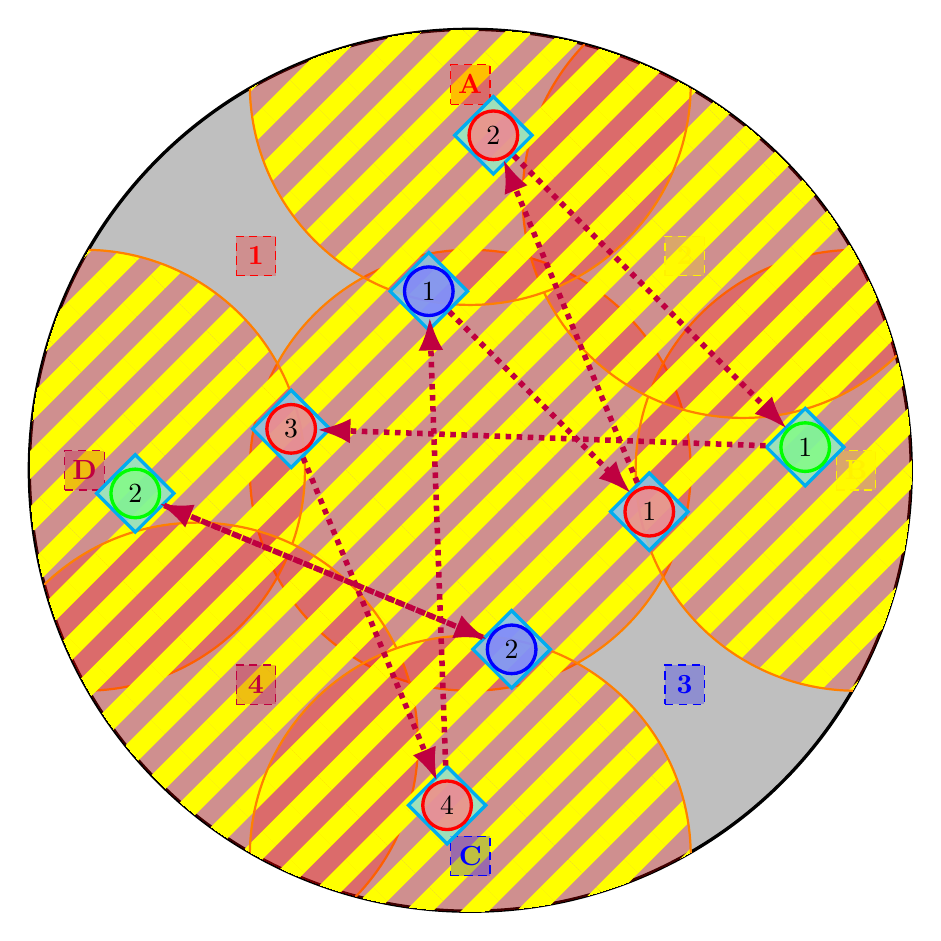
\begin{tikzpicture}[scale=1.4, every pic/.style={scale=1.4, transform shape}]
		% chktex-file 1
% chktex-file 8
\tikzset{arena/.style =
        {
            very thick,
            fill=gray,
            fill opacity=0.5
        }
}

\tikzset {marker/.style =
        {
            rectangle,
            densely dashed,
            minimum size=0.5cm,
            inner sep=0cm,
            text opacity=1,
            draw
        }
}

\tikzset{aoe/.style =
        {
            thick,
            orange,
            pattern={
                    Lines[angle=45, distance=0.5cm, line width=0.25cm]
                },
            pattern color=yellow,
            opacity=0.25,
            draw opacity=1
        }
}

\tikzset{aoe fill/.style = {
            fill=red,
            opacity=0.25
        }
}

\tikzset{cone aoe/.pic = {
            \draw [preaction={aoe fill}] [aoe] (0,0) -- (#1/2:10) arc (#1:-1*#1:5) -- cycle;
        }
}

\tikzset{line aoe/.pic = {
            \draw [preaction={aoe fill}] [aoe] (0,-0.5*#1) rectangle (10,0.5*#1);
        }
}

\tikzset{circle aoe/.pic = {
            \draw [preaction={aoe fill}] [aoe] (0,0) circle [radius=#1];
        }
}

\tikzset{pics/donut aoe/.style 2 args = {
            code = {
                    \draw [preaction={even odd rule,aoe fill}] [even odd rule,aoe] (0,0) circle [radius=#1] circle [radius=#2];
                }
        }
}

\tikzset{boss/.style =
        {
            shape=circle,
            very thick,
            purple,
            fill=purple!50,
            fill opacity=0.75,
            minimum size=1cm,
            text=black,
            text opacity=1,
            draw
        }
}

\tikzset{tank/.style =
        {
            boss,
            draw=blue,
            fill=blue!50,
            minimum size=0.5cm
        }
}

\tikzset{dps/.style =
        {
            tank,
            draw=red,
            fill=red!50
        }
}

\tikzset{heal/.style =
        {
            tank,
            draw=green,
            fill=green!50
        }
}

\tikzset{endat/.style =
        {
            shape=circle,
            very thick,
            draw=black,
            fill=black!50,
            minimum size=0.5cm
        }
}

\tikzset{startat/.style =
        {
            endat,
            dashed
        }
}

\tikzset{nf/.style = { fill=none } }

\tikzset{move/.style = {
            line width=2pt,
            -Latex,
            fill=none
        }
}

\tikzset{tether/.style = {
        line width=2pt,
        purple,
        dotted,
        -Latex,
        text=black
    }
}

\tikzset{icicle/.style =
        {
            shape=diamond,
            very thick,
            cyan,
            fill=cyan!50,
            fill opacity=0.75,
            minimum size=1cm,
            text=black,
            text opacity=1,
            draw
        }
}
		\foreach \letter / \ang / \rad / \c in
			{A/90/3.5/red,
				D/180/3.5/purple,
				C/270/3.5/blue,
				B/0/3.5/yellow,
				1/135/2.75/red,
				4/225/2.75/purple,
				3/315/2.75/blue,
				2/45/2.75/yellow}
		\node[marker, color=\c, fill, fill opacity=0.25] at (\ang:\rad) (marker-\letter) {\textbf\letter};

		\node[startat, below left=0cm of marker-2, draw=none, fill=none] (g1) {};
		\node[startat, above right=0cm of marker-4, draw=none, fill=none] (g2) {};

		\begin{scope}[name prefix=ice-, every node/.style = icicle]
			\path [rotate around={135:(g1)}] (g1)
			+(180:2cm) node (h1) {}
			+(135:2cm) node (d1) {}
			+(45:2cm) node (t1) {}
			+(0:2cm) node (d2) {};

			\path [rotate around={-45:(g2)}] (g2)
			+(180:2cm) node (h2) {}
			+(135:2cm) node (d3) {}
			+(45:2cm) node (t2) {}
			+(0:2cm) node (d4) {};
		\end{scope}

		\foreach \start/\type/\lab in {t1/tank/1, t2/tank/2, h1/heal/1, h2/heal/2, d1/dps/1, d2/dps/2, d3/dps/3, d4/dps/4}
		\node [\type] at (ice-\start) (\start) {\lab};

		\begin{scope}[on background layer, transparency group]
			\draw[arena] (0,0) circle [radius=4];
			\clip (0,0) circle [radius=4];
			\begin{scope}[transparency group]
				\pic at (0,0) {circle aoe=2cm};
				\foreach \ang in {0, 45, 90, 180, 225, 270}
				\pic at (\ang:3.5) {circle aoe=2cm};
			\end{scope}
		\end{scope}

		\foreach \start / \finish in
			{ice-t1/d1,
				ice-t2/h2,
				ice-h1/d3,
				ice-h2/t2,
				ice-d1/d2,
				ice-d2/h1,
				ice-d3/d4,
				ice-d4/t1}
			{
				\draw [tether] (\start) -- (\finish);
			}


	\end{tikzpicture}
	\caption{Icicles drop, tethers are assigned, and a new safe spot appears}
	\label{icicledrop}
\end{figure}

\begin{figure}
	\centering
	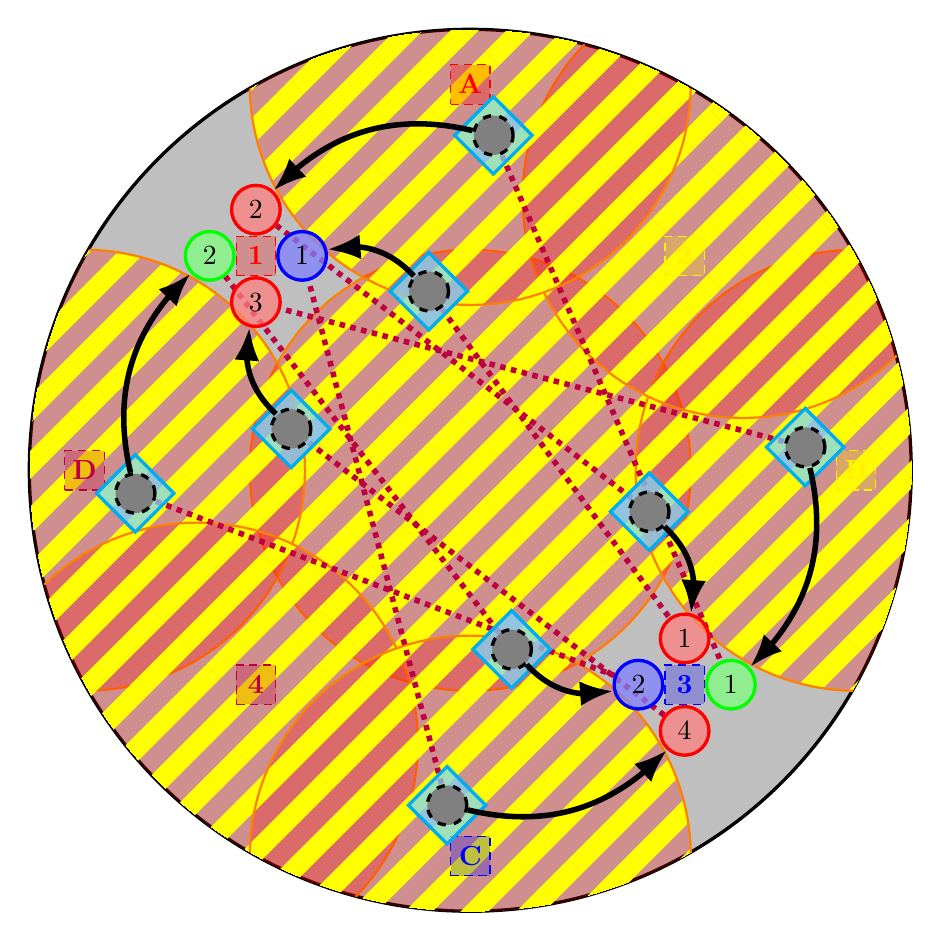
\begin{tikzpicture}[scale=1.4, every pic/.style={scale=1.4, transform shape}]
		% chktex-file 1
% chktex-file 8
\tikzset{arena/.style =
        {
            very thick,
            fill=gray,
            fill opacity=0.5
        }
}

\tikzset {marker/.style =
        {
            rectangle,
            densely dashed,
            minimum size=0.5cm,
            inner sep=0cm,
            text opacity=1,
            draw
        }
}

\tikzset{aoe/.style =
        {
            thick,
            orange,
            pattern={
                    Lines[angle=45, distance=0.5cm, line width=0.25cm]
                },
            pattern color=yellow,
            opacity=0.25,
            draw opacity=1
        }
}

\tikzset{aoe fill/.style = {
            fill=red,
            opacity=0.25
        }
}

\tikzset{cone aoe/.pic = {
            \draw [preaction={aoe fill}] [aoe] (0,0) -- (#1/2:10) arc (#1:-1*#1:5) -- cycle;
        }
}

\tikzset{line aoe/.pic = {
            \draw [preaction={aoe fill}] [aoe] (0,-0.5*#1) rectangle (10,0.5*#1);
        }
}

\tikzset{circle aoe/.pic = {
            \draw [preaction={aoe fill}] [aoe] (0,0) circle [radius=#1];
        }
}

\tikzset{pics/donut aoe/.style 2 args = {
            code = {
                    \draw [preaction={even odd rule,aoe fill}] [even odd rule,aoe] (0,0) circle [radius=#1] circle [radius=#2];
                }
        }
}

\tikzset{boss/.style =
        {
            shape=circle,
            very thick,
            purple,
            fill=purple!50,
            fill opacity=0.75,
            minimum size=1cm,
            text=black,
            text opacity=1,
            draw
        }
}

\tikzset{tank/.style =
        {
            boss,
            draw=blue,
            fill=blue!50,
            minimum size=0.5cm
        }
}

\tikzset{dps/.style =
        {
            tank,
            draw=red,
            fill=red!50
        }
}

\tikzset{heal/.style =
        {
            tank,
            draw=green,
            fill=green!50
        }
}

\tikzset{endat/.style =
        {
            shape=circle,
            very thick,
            draw=black,
            fill=black!50,
            minimum size=0.5cm
        }
}

\tikzset{startat/.style =
        {
            endat,
            dashed
        }
}

\tikzset{nf/.style = { fill=none } }

\tikzset{move/.style = {
            line width=2pt,
            -Latex,
            fill=none
        }
}

\tikzset{tether/.style = {
        line width=2pt,
        purple,
        dotted,
        -Latex,
        text=black
    }
}

\tikzset{icicle/.style =
        {
            shape=diamond,
            very thick,
            cyan,
            fill=cyan!50,
            fill opacity=0.75,
            minimum size=1cm,
            text=black,
            text opacity=1,
            draw
        }
}
		\foreach \letter / \ang / \rad / \c in
			{A/90/3.5/red,
				D/180/3.5/purple,
				C/270/3.5/blue,
				B/0/3.5/yellow,
				1/135/2.75/red,
				4/225/2.75/purple,
				3/315/2.75/blue,
				2/45/2.75/yellow}
		\node[marker, color=\c, fill, fill opacity=0.25] at (\ang:\rad) (marker-\letter) {\textbf\letter};

		\node[startat, below left=0cm of marker-2, draw=none, fill=none] (g1) {};
		\node[startat, above right=0cm of marker-4, draw=none, fill=none] (g2) {};

		\begin{scope}[name prefix=ice-, every node/.style = icicle]
			\path [rotate around={135:(g1)}] (g1)
			+(180:2cm) node (h1) {}
			+(135:2cm) node (d1) {}
			+(45:2cm) node (t1) {}
			+(0:2cm) node (d2) {};

			\path [rotate around={-45:(g2)}] (g2)
			+(180:2cm) node (h2) {}
			+(135:2cm) node (d3) {}
			+(45:2cm) node (t2) {}
			+(0:2cm) node (d4) {};
		\end{scope}

		\foreach \start/\type/\lab in {t1/tank/1, t2/tank/2, h1/heal/1, h2/heal/2, d1/dps/1, d2/dps/2, d3/dps/3, d4/dps/4}
		\node[startat] (prev-\start) at (ice-\start) {};

		\node[heal, right=0cm of marker-3] (h1) {1};
		\node[heal, left=0cm of marker-1] (h2) {2};
		\node[tank, right=0cm of marker-1] (t1) {1};
		\node[tank, left=0cm of marker-3] (t2) {2};
		\node[dps, above=0cm of marker-3] (d1) {1};
		\node[dps, above=0cm of marker-1] (d2) {2};
		\node[dps, below=0cm of marker-1] (d3) {3};
		\node[dps, below=0cm of marker-3] (d4) {4};

		\begin{scope}[on background layer, transparency group]
			\draw[arena] (0,0) circle [radius=4];
			\clip (0,0) circle [radius=4];
			\begin{scope}[transparency group]
				\pic at (0,0) {circle aoe=2cm};
				\foreach \ang in {0, 45, 90, 180, 225, 270}
				\pic at (\ang:3.5) {circle aoe=2cm};
			\end{scope}

			\foreach \start / \finish in
				{ice-t1/d1,
					ice-t2/h2,
					ice-h1/d3,
					ice-h2/t2,
					ice-d1/d2,
					ice-d2/h1,
					ice-d3/d4,
					ice-d4/t1}
				{
					\draw [tether, -] (\start.center) -- (\finish);
				}
		\end{scope}


		\foreach \player in {h1,h2,d1,d3}
		\draw [move, bend left] (prev-\player) to (\player);
		\foreach \player in {t1,t2,d2,d4}
		\draw [move, bend right] (prev-\player) to (\player);

	\end{tikzpicture}
	\caption{Tethered players move to the safe spots}
	\label{secondsafespot}
\end{figure}

\section{Preparing to resolve the tethers}

Once all the current AOEs are resolved, all players move to the center of the arena, arranging themselves around the center point so that the center is between them and their tethered icicle.  All players need to use knockback mitigation here.

\begin{figure}[h]
	\centering
	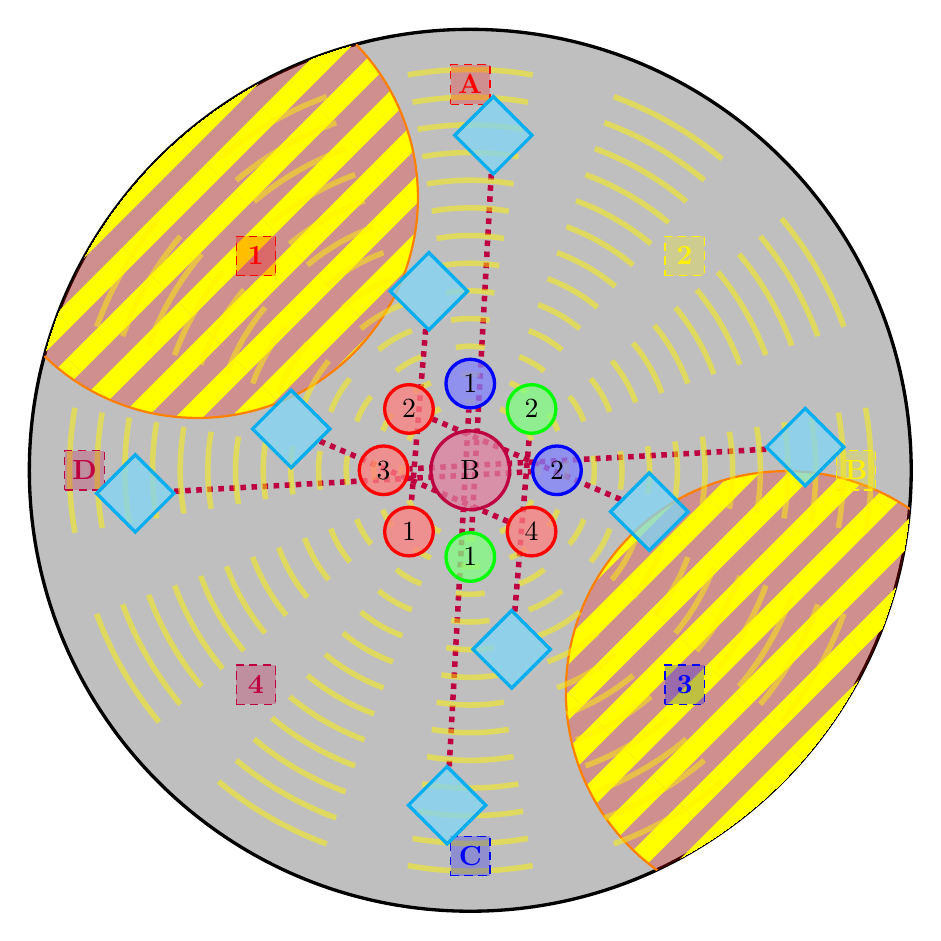
\begin{tikzpicture}[scale=1.4, every pic/.style={scale=1.4, transform shape}]
		% chktex-file 1
% chktex-file 8
\tikzset{arena/.style =
        {
            very thick,
            fill=gray,
            fill opacity=0.5
        }
}

\tikzset {marker/.style =
        {
            rectangle,
            densely dashed,
            minimum size=0.5cm,
            inner sep=0cm,
            text opacity=1,
            draw
        }
}

\tikzset{aoe/.style =
        {
            thick,
            orange,
            pattern={
                    Lines[angle=45, distance=0.5cm, line width=0.25cm]
                },
            pattern color=yellow,
            opacity=0.25,
            draw opacity=1
        }
}

\tikzset{aoe fill/.style = {
            fill=red,
            opacity=0.25
        }
}

\tikzset{cone aoe/.pic = {
            \draw [preaction={aoe fill}] [aoe] (0,0) -- (#1/2:10) arc (#1:-1*#1:5) -- cycle;
        }
}

\tikzset{line aoe/.pic = {
            \draw [preaction={aoe fill}] [aoe] (0,-0.5*#1) rectangle (10,0.5*#1);
        }
}

\tikzset{circle aoe/.pic = {
            \draw [preaction={aoe fill}] [aoe] (0,0) circle [radius=#1];
        }
}

\tikzset{pics/donut aoe/.style 2 args = {
            code = {
                    \draw [preaction={even odd rule,aoe fill}] [even odd rule,aoe] (0,0) circle [radius=#1] circle [radius=#2];
                }
        }
}

\tikzset{boss/.style =
        {
            shape=circle,
            very thick,
            purple,
            fill=purple!50,
            fill opacity=0.75,
            minimum size=1cm,
            text=black,
            text opacity=1,
            draw
        }
}

\tikzset{tank/.style =
        {
            boss,
            draw=blue,
            fill=blue!50,
            minimum size=0.5cm
        }
}

\tikzset{dps/.style =
        {
            tank,
            draw=red,
            fill=red!50
        }
}

\tikzset{heal/.style =
        {
            tank,
            draw=green,
            fill=green!50
        }
}

\tikzset{endat/.style =
        {
            shape=circle,
            very thick,
            draw=black,
            fill=black!50,
            minimum size=0.5cm
        }
}

\tikzset{startat/.style =
        {
            endat,
            dashed
        }
}

\tikzset{nf/.style = { fill=none } }

\tikzset{move/.style = {
            line width=2pt,
            -Latex,
            fill=none
        }
}

\tikzset{tether/.style = {
        line width=2pt,
        purple,
        dotted,
        -Latex,
        text=black
    }
}

\tikzset{icicle/.style =
        {
            shape=diamond,
            very thick,
            cyan,
            fill=cyan!50,
            fill opacity=0.75,
            minimum size=1cm,
            text=black,
            text opacity=1,
            draw
        }
}
		\foreach \letter / \ang / \rad / \c in
			{A/90/3.5/red,
				D/180/3.5/purple,
				C/270/3.5/blue,
				B/0/3.5/yellow,
				1/135/2.75/red,
				4/225/2.75/purple,
				3/315/2.75/blue,
				2/45/2.75/yellow}
		\node[marker, color=\c, fill, fill opacity=0.25] at (\ang:\rad) (marker-\letter) {\textbf\letter};

		\node[boss] (boss) at (0,0) {B};

		\node[startat, below left=0cm of marker-2, draw=none, fill=none] (g1) {};
		\node[startat, above right=0cm of marker-4, draw=none, fill=none] (g2) {};

		\begin{scope}[name prefix=ice-, every node/.style = icicle]
			\path [rotate around={135:(g1)}] (g1)
			+(180:2cm) node (h1) {}
			+(135:2cm) node (d1) {}
			+(45:2cm) node (t1) {}
			+(0:2cm) node (d2) {};

			\path [rotate around={-45:(g2)}] (g2)
			+(180:2cm) node (h2) {}
			+(135:2cm) node (d3) {}
			+(45:2cm) node (t2) {}
			+(0:2cm) node (d4) {};
		\end{scope}

		\begin{scope}[node distance=0.25cm]
			\node[heal, below=of boss] (h1) {1};
			\node[heal, above right=of boss] (h2) {2};
			\node[tank, above=of boss] (t1) {1};
			\node[tank, right=of boss] (t2) {2};
			\node[dps, below left=of boss] (d1) {1};
			\node[dps, above left=of boss] (d2) {2};
			\node[dps, left=of boss] (d3) {3};
			\node[dps, below right=of boss] (d4) {4};
		\end{scope}

		\begin{scope}[on background layer, transparency group]
			\draw[arena] (0,0) circle [radius=4];
			\clip (0,0) circle [radius=4];

			\foreach \start / \finish in
				{ice-t1/d1,
					ice-t2/h2,
					ice-h1/d3,
					ice-h2/t2,
					ice-d1/d2,
					ice-d2/h1,
					ice-d3/d4,
					ice-d4/t1}
				{
					\draw [tether, -] (\start) -- (\finish);
				}

			\begin{scope}[transparency group]
				\foreach \ang in {135, 325}
				\pic at (\ang:3.5) {circle aoe=2cm};
			\end{scope}

			\foreach \ang in {0, 30, ..., 359}
			\draw [line width=2pt, opacity=0.5, yellow,
				decorate,
				decoration={expanding waves, angle=10}]
			(boss) -- ++(\ang:3.75);
		\end{scope}

	\end{tikzpicture}
	\caption{Players gather in the center, getting ready to resolve their tethers while avoiding the remaining two AOEs}
	\label{prepforknockback}
\end{figure}

\section{Clean up and resolve tethers}

After the final two AOEs resolve, players move to the outside of the arena.  There is enough time for players to adjust to make sure that they are not in the path of other tethered icicles, or that their icicles do not hit other players.  After the tethers resolve, this completes the \emph{Junction Shiva} phase.

\begin{figure}[h]
	\centering
	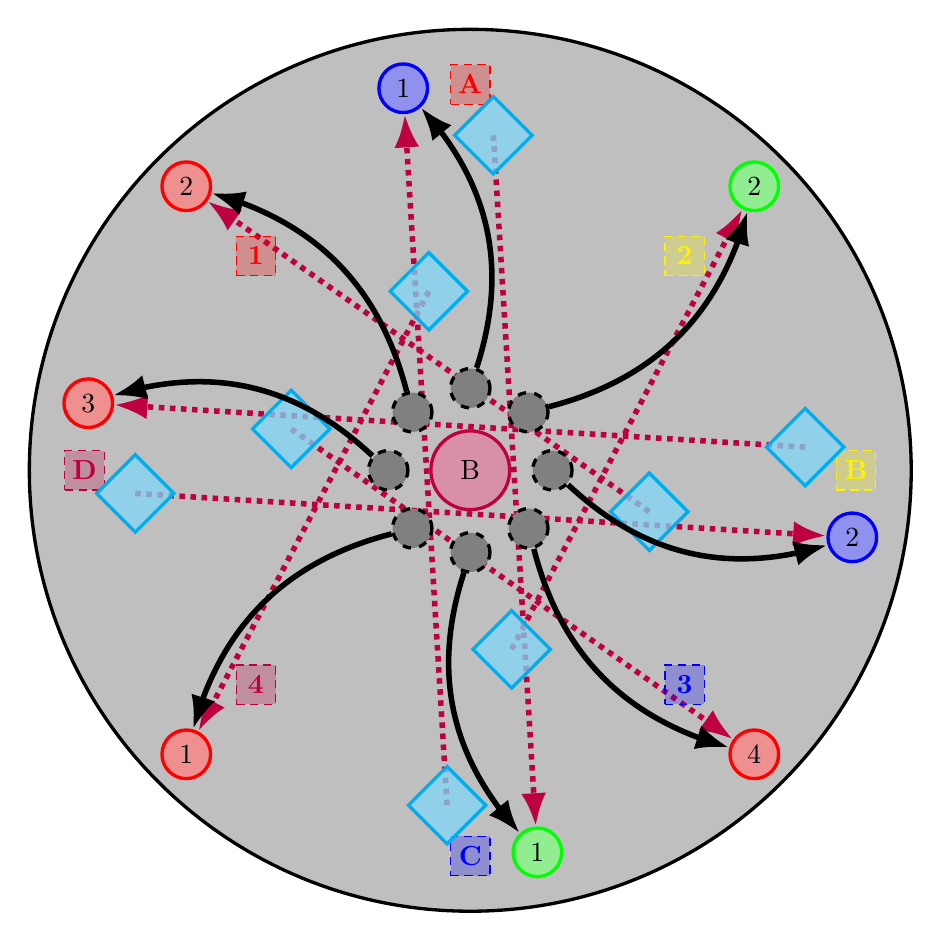
\begin{tikzpicture}[scale=1.4, every pic/.style={scale=1.4, transform shape}]
		% chktex-file 1
% chktex-file 8
\tikzset{arena/.style =
        {
            very thick,
            fill=gray,
            fill opacity=0.5
        }
}

\tikzset {marker/.style =
        {
            rectangle,
            densely dashed,
            minimum size=0.5cm,
            inner sep=0cm,
            text opacity=1,
            draw
        }
}

\tikzset{aoe/.style =
        {
            thick,
            orange,
            pattern={
                    Lines[angle=45, distance=0.5cm, line width=0.25cm]
                },
            pattern color=yellow,
            opacity=0.25,
            draw opacity=1
        }
}

\tikzset{aoe fill/.style = {
            fill=red,
            opacity=0.25
        }
}

\tikzset{cone aoe/.pic = {
            \draw [preaction={aoe fill}] [aoe] (0,0) -- (#1/2:10) arc (#1:-1*#1:5) -- cycle;
        }
}

\tikzset{line aoe/.pic = {
            \draw [preaction={aoe fill}] [aoe] (0,-0.5*#1) rectangle (10,0.5*#1);
        }
}

\tikzset{circle aoe/.pic = {
            \draw [preaction={aoe fill}] [aoe] (0,0) circle [radius=#1];
        }
}

\tikzset{pics/donut aoe/.style 2 args = {
            code = {
                    \draw [preaction={even odd rule,aoe fill}] [even odd rule,aoe] (0,0) circle [radius=#1] circle [radius=#2];
                }
        }
}

\tikzset{boss/.style =
        {
            shape=circle,
            very thick,
            purple,
            fill=purple!50,
            fill opacity=0.75,
            minimum size=1cm,
            text=black,
            text opacity=1,
            draw
        }
}

\tikzset{tank/.style =
        {
            boss,
            draw=blue,
            fill=blue!50,
            minimum size=0.5cm
        }
}

\tikzset{dps/.style =
        {
            tank,
            draw=red,
            fill=red!50
        }
}

\tikzset{heal/.style =
        {
            tank,
            draw=green,
            fill=green!50
        }
}

\tikzset{endat/.style =
        {
            shape=circle,
            very thick,
            draw=black,
            fill=black!50,
            minimum size=0.5cm
        }
}

\tikzset{startat/.style =
        {
            endat,
            dashed
        }
}

\tikzset{nf/.style = { fill=none } }

\tikzset{move/.style = {
            line width=2pt,
            -Latex,
            fill=none
        }
}

\tikzset{tether/.style = {
        line width=2pt,
        purple,
        dotted,
        -Latex,
        text=black
    }
}

\tikzset{icicle/.style =
        {
            shape=diamond,
            very thick,
            cyan,
            fill=cyan!50,
            fill opacity=0.75,
            minimum size=1cm,
            text=black,
            text opacity=1,
            draw
        }
}
		\foreach \letter / \ang / \rad / \c in
			{A/90/3.5/red,
				D/180/3.5/purple,
				C/270/3.5/blue,
				B/0/3.5/yellow,
				1/135/2.75/red,
				4/225/2.75/purple,
				3/315/2.75/blue,
				2/45/2.75/yellow}
		\node[marker, color=\c, fill, fill opacity=0.25] at (\ang:\rad) (marker-\letter) {\textbf\letter};

		\node[boss] (boss) at (0,0) {B};

		\node[startat, below left=0cm of marker-2, draw=none, fill=none] (g1) {};
		\node[startat, above right=0cm of marker-4, draw=none, fill=none] (g2) {};

		\begin{scope}[name prefix=ice-, every node/.style = icicle]
			\path [rotate around={135:(g1)}] (g1)
			+(180:2cm) node (h1) {}
			+(135:2cm) node (d1) {}
			+(45:2cm) node (t1) {}
			+(0:2cm) node (d2) {};

			\path [rotate around={-45:(g2)}] (g2)
			+(180:2cm) node (h2) {}
			+(135:2cm) node (d3) {}
			+(45:2cm) node (t2) {}
			+(0:2cm) node (d4) {};
		\end{scope}

		\begin{scope}[node distance=0.25cm, name prefix=prev-, every node/.style = startat]
			\node[below=of boss] (h1) {};
			\node[above right=of boss] (h2) {};
			\node[above=of boss] (t1) {};
			\node[right=of boss] (t2) {};
			\node[below left=of boss] (d1) {};
			\node[above left=of boss] (d2) {};
			\node[left=of boss] (d3) {};
			\node[below right=of boss] (d4) {};
		\end{scope}

		\begin{scope}[node distance=4.25cm]
			\node[heal, below right=4.25cm and 0.25cm of boss] (h1) {1};
			\node[heal, above right=of boss] (h2) {2};
			\node[tank, above left=4.25cm and 0.25cm of boss] (t1) {1};
			\node[tank, below right=0.25cm and 4.25cm of boss] (t2) {2};
			\node[dps, below left=of boss] (d1) {1};
			\node[dps, above left=of boss] (d2) {2};
			\node[dps, above left=0.25cm and 4.25cm of boss] (d3) {3};
			\node[dps, below right=of boss] (d4) {4};
		\end{scope}

		\begin{scope}[on background layer, transparency group]
			\draw[arena] (0,0) circle [radius=4];
			\clip (0,0) circle [radius=4];

			\foreach \start / \finish in
				{ice-t1/d1,
					ice-t2/h2,
					ice-h1/d3,
					ice-h2/t2,
					ice-d1/d2,
					ice-d2/h1,
					ice-d3/d4,
					ice-d4/t1}
				{
					\draw [tether] (\start.center) -- (\finish);
				}
		\end{scope}

		\foreach \player in {h1,h2,d1,d3,t1,t2,d2,d4}
		\draw [move, bend right] (prev-\player) to (\player);

	\end{tikzpicture}
	\caption{Players move to the outside edge of the arena and adjust so that everybody is hit by only one icicle}
	\label{resolve}
\end{figure}

\end{document}